\section{Results}
\label{sec:results}

Tbl.~\ref{tab:results} presents the full benchmark results.
Reliability (success rate), speed (median settling time), and control effort do not order the controllers the same way: the most reliable are also among the fastest, but others trade speed for reliability or, like IQL, speed for gentleness.
The three data-driven controllers (MPPI, PPO-WM, IQL) post the highest mean reliability (97\%) of any family, and the lowest mean effort (0.41), roughly 30\% below the classical and simulation-trained families.
At the other extreme, the highest-effort controllers, TD3 and TQC (RMS effort 0.68 and 0.66), run close to the $\pm 0.9$~m/s saturation limit and drive the actuator into saturation on many trials.
Three findings below explain these differences, and a closing note covers offline RL.

\begin{table*}[t]
\centering
\caption{Hardware benchmark results (50 trials per controller, 20\,Hz).
  SR = success rate with 95\% Wilson score CI; settling statistics computed over successful trials only.
  RMS effort is the root-mean-square commanded cart velocity (m/s),
  saturated at the $\pm 0.9$~m/s axis limit.
  Data source / mechanism follows the two-axis taxonomy of Tbl.~\ref{tab:controllers}.
  Sorted by SR, then by mean settling time.}
\label{tab:results}
\begin{tabular}{llccccc}
\toprule
\textbf{Controller} & \textbf{Data source / mechanism} & \textbf{SR (\%)} & \textbf{95\% CI}
  & \textbf{Mean (s)} & \textbf{Median (s) [IQR]} & \textbf{RMS Effort} \\
\midrule
MPPI         & Logged data / sampling MPC & \textbf{100} & [93, 100] & \textbf{2.06} & \textbf{1.67}\,[1.04, 2.67] & \textbf{0.354} \\
PPO (WM)     & Logged data / trained-in-model RL & \textbf{100} & [93, 100] & 6.84 & 3.64\,[2.04, 7.54] & 0.492 \\
PPO (BZ+DR)  & Sim / model-free RL    & 96 & [87, 99]   & 3.81 & 3.15\,[1.29, 4.96] & 0.498 \\
PD + WO      & Analytical / error feedback & 96 & [87, 99]  & 5.80 & 3.38\,[1.11, 7.48] & 0.580 \\
\midrule
SMC + WO     & Analytical / sliding-mode & 92 & [81, 97]   & 8.93  & 8.28\,[4.69, 10.78]  & 0.562 \\
LQR + WO     & Analytical / PD-equivalent feedback & 92 & [81, 97]   & 10.21 & 8.28\,[2.86, 16.68]  & 0.625 \\
IQL          & Logged data / offline RL   & 92 & [81, 97]   & 10.62 & 9.80\,[4.49, 15.63]  & 0.395 \\
TD3 (DR)     & Sim / model-free RL    & 92 & [81, 97]   & 11.45 & 10.06\,[4.54, 17.91] & 0.680 \\
NMPC         & Analytical / nonlinear MPC & 90 & [79, 96]   & 7.48  & 4.71\,[1.35, 7.51]   & 0.608 \\
TRPO (DR)    & Sim / model-free RL    & 90 & [79, 96]   & 8.09  & 4.80\,[1.50, 13.60]  & 0.508 \\
\midrule
TQC (DR)     & Sim / model-free RL    & 86 & [74, 93]   & 9.77  & 6.61\,[2.68, 15.51]  & 0.663 \\
SAC (DR)     & Sim / model-free RL    & 82 & [69, 90]   & 10.10 & 8.40\,[3.26, 15.16]  & 0.588 \\
MPC + WO     & Analytical / linear MPC & 80 & [67, 89]   & 10.81 & 9.65\,[2.35, 18.35]  & 0.623 \\
\bottomrule
\end{tabular}
\end{table*}

\subsection{Constraint Handling and the Choice of Paradigm}

The comparison's central result is a difference in magnitude: handling the rail boundary changes reliability a great deal, while any effect of the control paradigm is too small for this protocol to resolve.
The deployed LQR, run without boundary handling, succeeds on only 20\% of hardware trials: it corrects the ball but lets the cart drift into the rail, and cannot recover from there.
Adding a wall override, with the gain unchanged, raises it to 92\%.
The CMA-ES-tuned gain reached only 16\% even with the override; the supplement reports that comparison.
This override rule, run over the 50-trial protocol, lifts every classical controller into the reliable group:

\begin{center}
\begin{tabular}{lcc}
\toprule
 & Without WO & With WO \\
\midrule
PD & 18\% & 96\% (+78\,pp) \\
LQR & 20\% & 92\% (+72\,pp) \\
SMC & 12\% & 92\% (+80\,pp) \\
\bottomrule
\end{tabular}
\end{center}

Against a change of this size, any effect of the paradigm behind a controller is small enough that this protocol cannot resolve it.
The controllers at 90\% success or better come from all four families, and no pairwise success-rate difference within this group is statistically significant (Fisher's exact test, Bonferroni corrected).
The two lowest, MPC+WO at 80\% and SAC at 82\%, may well be less reliable, but with fifty trials and correction across every pair we cannot establish it.
NMPC reaches the reliable group through its own internal constraint handling (45/50), with no external override.

Control effort is the one axis on which the benchmark does resolve a paradigm difference: 58 of the 78 pairwise RMS-effort differences are significant (Mann-Whitney, Bonferroni corrected as its own family).
MPPI and IQL, the two lowest-effort controllers, each use significantly less effort than every other controller except one another, holding their reliability while keeping the actuator clear of the saturation the wall-override controllers reach by design.
PPO-WM, whose learned model carries only a weak action response, sits mid-range, its effort not separable from PPO~(BZ+DR) or TRPO.

Fig.~\ref{fig:pareto} places all 13 on the speed-reliability plane.
MPPI ties for the highest success rate and settles fastest; its edge over the other reliable controllers is one of speed alone.
Its settling time is significantly shorter than nine of the twelve other controllers, while against PPO~(BZ+DR), PD+WO, and NMPC the difference stays below significance at this sample size (the effect sizes are given in the supplement).

\subsection{Two Deployments from a Learned Model}

A small LSTM trained on logged hardware data captures dynamics our analytical model misses (the supplement shows it has lower total trajectory error at every tested horizon).
A learned model of this kind enables two deployment strategies with different cost profiles.

\noindent\textbf{Online planning (MPPI):} Using the learned model for sampling-based planning at every timestep achieves the best combined performance: 100\% success, fastest median settling (1.67\,s), and lowest control effort (0.354 RMS), at the cost of real-time model rollouts (mean 40\,ms per step on CPU, within the 50\,ms control period after a one-step cold start; the supplement gives the full timing distribution and a 2$\times$ speedup on 4 threads).

\noindent\textbf{Offline policy training (PPO-WM):} Training an RL policy inside a learned model of the same kind reaches the same 100\% reliability with about 6.7\,ms CPU inference per step, cheaper than MPPI's $\sim$40\,ms planning; PPO-WM trains and deploys on CPU ($\sim$42\,min training), no GPU needed.
PPO-WM's world model is built from a different logged collection than the one MPPI plans through; the supplement details both.

\noindent\textbf{How much data is needed?} An open-loop data sweep shows prediction error plateauing around 50--100k transitions.
In open loop, an accurate model needs far less data than the 1M we collected, though how much accuracy survives closed-loop deployment depends on the planner.

MPPI's speed advantage also shows up as consistency: in the settling-time distributions of Fig.~\ref{fig:boxplot}, its spread is the tightest of any controller, with every successful trial settling in a few seconds and none past 9\,s.
The wall-override classical controllers are more spread out, fast when the ball stays clear of the boundary and slow when the override has to bring it back from the rail.

The supplementary material breaks settling time down by the cart's starting stratum.
The clearest pattern there is MPPI's consistency across strata; the other controllers vary more, though with only five trials in each at-wall stratum those per-controller differences are descriptive rather than tested.

\begin{figure}[t]
  \centering
  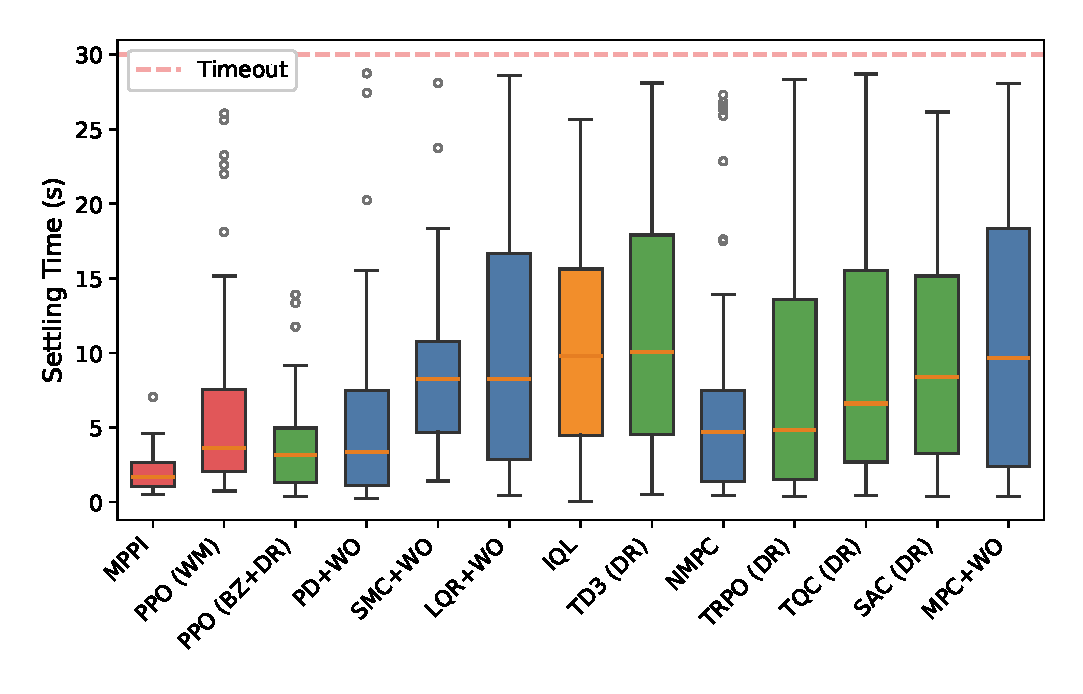
\includegraphics[width=0.95\columnwidth]{figures/exp1_boxplot.eps}
  \caption{Settling time distributions. MPPI shows the tightest
    distribution with no outliers beyond 9\,s. Classical controllers
    with wall override show bimodal behavior: fast successes plus
    occasional slow recoveries after the override triggers.}
  \label{fig:boxplot}
\end{figure}

\begin{figure}[t]
  \centering
  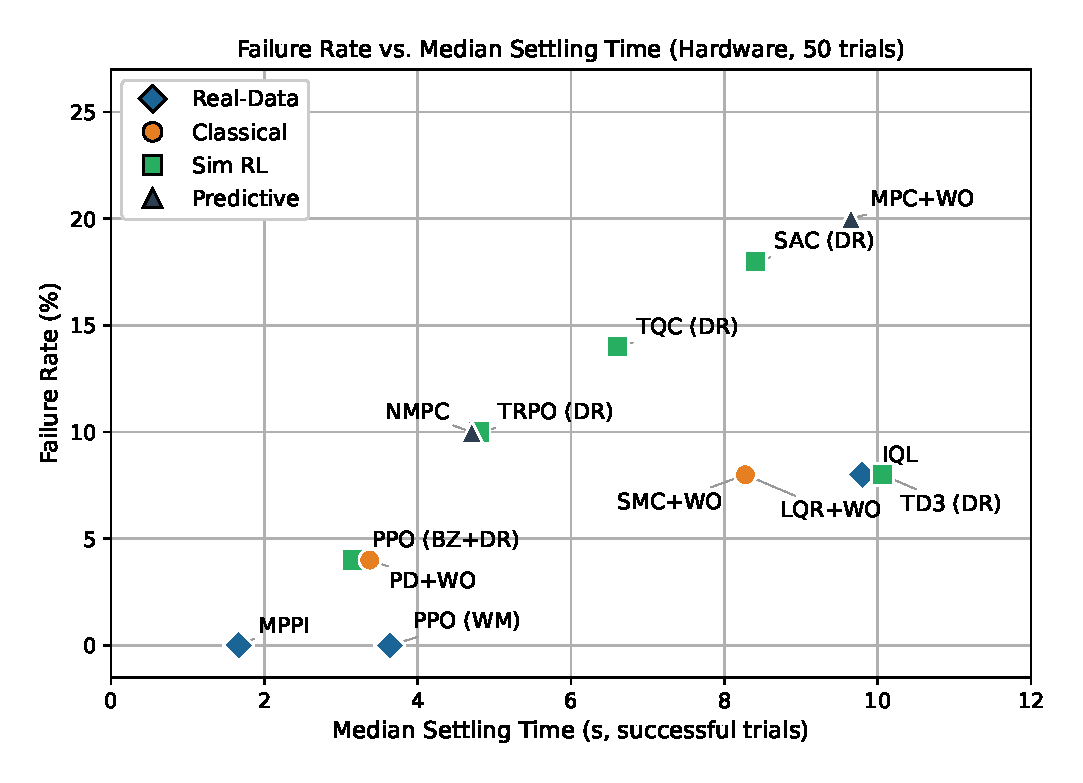
\includegraphics[width=0.95\columnwidth]{figures/hw_sr_vs_settling.eps}
  \caption{Failure rate versus median settling time (successful
    trials) across all 13 controllers. Both axes increase toward worse
    outcomes, so the ideal corner is bottom-left. MPPI ties for the best
    success rate and is fastest on median settling (100\%, 1.67\,s). Two
    controllers achieve perfect reliability; all handle the boundary,
    whether explicitly or through learned dynamics.}
  \label{fig:pareto}
\end{figure}

\subsection{The Reach of Domain Randomization}

Domain randomization is the workhorse of sim-to-real transfer~\cite{zhao2020simtoreal}, and has carried policies onto hardware as demanding as in-hand manipulation and champion-level drone racing.
In our PPO ablation it does most of the work and then plateaus: it lifts hardware success from 60\% without it to 90\% with it, a thirty-point gain, after which the remaining gap did not close with more of it.

The source of the remaining gap is less certain.
We can model one sensor effect directly: near the arc edges the ToF sensors saturate and report frozen values, and a policy trained without this artifact overcorrects on stale data.
Adding a blind-zone model lifts PPO from 90\% to 98\%.\footnote{The domain-randomization and blind-zone ablations in this subsection are measured within the S-curve servo-model family, the regime the extended training runs used. Tbl.~\ref{tab:results} instead reports PPO~(BZ+DR) at the first-order-lag checkpoint (96\%), matched to the servo model the other 4 RL agents trained against so the cross-agent comparison is fair; the supplement reports both.} At 50 trials this eight-point move is within the benchmark's resolution, so we treat the perceptual reading as a hypothesis; the data cannot yet resolve an effect this small.
Nor is modeling the sensor the only route past the plateau: trained to 5M steps, the base PPO policy also reaches 100\% over 50 hardware trials, so the blind-zone model is the training-efficient path rather than the necessary one.
It fits what we see: the five simulation-trained RL agents all reach 96--100\% in simulation yet span only 82\% to 96\% on hardware, though they also differ in their training conditions, so this cross-agent spread is suggestive and not conclusive.

\subsection{A Note on Offline RL}

IQL achieves 92\% success at the second-lowest control effort of any controller (0.395 RMS, behind only MPPI), using no simulator: its conservative policy is reliable and gentle on the hardware, at the price of speed, with a median settling of 9.80\,s, roughly six times MPPI's.
The result is attractive mainly for where the data came from: the dataset built up as a by-product of normal evaluation runs, so once a platform is instrumented and several controllers have been run, offline RL becomes a viable low-overhead option when simulation fidelity is uncertain.
